\section{Network Characterization}\label{sec:NC}
All metrics in this section use the undirected, unweighted projections of $G_{Cit}$ and $G_{BC}$ defined in Section~\ref{sec:DC}; directed and weighted variants enter only when explicitly noted.

\begin{table*}[t]
\centering
\resizebox{\linewidth}{!}{%
\begin{tabular}{@{}l ccc ccc ccccccc ccccc@{}}
\toprule
 & \multicolumn{3}{c}{Full graph}
 & \multicolumn{3}{c}{LCC}
 & \multicolumn{7}{c}{Degree (LCC)}
 & \multicolumn{5}{c}{Clustering \& paths (LCC)} \\
\cmidrule(r){2-4}\cmidrule(lr){5-7}\cmidrule(lr){8-14}\cmidrule(l){15-19}
 & $N$ & $E$ & \#CC
 & $N$ & $E$ & Cov.
 & Mean & Std & Med & Max & P99 & $k{=}1$\,(\%)
 & Avg\,$C$ & Med\,$C$ & $C{=}0$\,(\%) & Density & $L$ & Diam. \\
\midrule
$G_{Cit}$
  & 55\,078 & 217\,174 & 1\,488
  & 49\,243 & 209\,599 & 89.4\%
  &  8.51 & 10.78 &  6 &   621 &  41 & 10.4
  & 0.342 & 0.321 & 21.4 & $1.7{\times}10^{-4}$ & 11.81 & 48 \\
$G_{BC}$
  & 57\,603 & 745\,451 & 1\,168
  & 53\,405 & 739\,498 & 92.7\%
  & 27.69 & 103.21 & 8 & 1\,169 & 726 &  7.8
  & 0.425 & 0.400 & 14.7 & $5.2{\times}10^{-4}$ & 10.04 & 33 \\
\bottomrule
\end{tabular}%
}
\caption{Structural summary of $G_{Cit}$ and $G_{BC}$.
Neither graph contains isolated nodes by construction.
$C{=}0$: fraction of nodes with zero clustering; std.\ of $C$ is $0.284$ for both graphs;
$L$: mean geodesic (NetworKit, exact).}
\label{tab:summary}
\end{table*}

Of $G_{BC}$'s edges, 70.9\% come from BC alone, 19.5\% from direct citation, and 9.7\% carry both signals---so BC-only edges outnumber citation-only edges $3.64\times$. 

The structural effect is visible in Table~\ref{tab:summary}: component count drops by 320 and LCC coverage rises by 3.3~pp, as shared references stitch together fragments that citation links leave isolated. These component-level shifts propagate differently across degree, clustering, and path structure:

\begin{itemize}
  \item \textbf{Degree.} BC more than triples average degree, but the effect concentrates in the upper tail: P99 jumps from 41 to 726 and standard deviation grows tenfold, while the median shifts only from 6 to 8. The fraction of degree-one nodes drops modestly (10.4\% $\to$ 7.8\%). Both distributions show a heavy tail well beyond the ER cutoff, closer in shape to the BA model (Figure~\ref{fig:degree_null}): $G_{BC}$'s fitted exponent ($\hat{\gamma}=2.13$) is shallower than $G_{Cit}$'s ($\hat{\gamma}=3.54$), though neither CCDF is strictly linear on a log-log scale.

  \item \textbf{Clustering and density.} BC triples density ($3.00\times$) but raises average clustering by only $1.24\times$---most BC edges bridge across neighbourhoods rather than close triangles within them. Zero-clustering nodes fall from 21.4\% to 14.7\%.

  \item \textbf{Path structure.} BC reduces mean geodesic by 15.0\% ($11.81 \to 10.04$) and diameter from 48 to 33---unlike clustering, both the bulk and the extremes of the distance distribution contract. Both averages remain high relative to the ER baseline ($L_{ER} = 3.65$ for $G_{BC}$, $5.30$ for $G_{Cit}$).
\end{itemize}

\subsection{Comparison with Random Graph Models}\label{sec:null}

Table~\ref{tab:null} details those baselines: Erd\H{o}s--R\'enyi $G(N,E)$ matched exactly on edge count, and Barab\'asi--Albert ($m=14$ for $G_{BC}$, $m=4$ for $G_{Cit}$), with a $\pm$1--6\% edge-count mismatch that does not affect the qualitative comparison.

Clustering exceeds ER by $850\times$ for $G_{BC}$ and $1{,}700\times$ for $G_{Cit}$, while mean path length is only $2.2$--$2.8\times$ longer---yielding $\sigma = 290.97$ and $808.71$, far above the $\sigma > 1$ threshold. At citation-graph density, ER falls just below the full-connectivity threshold ($\langle k \rangle = 8.51 < \ln N \approx 10.8$), leaving 12 nodes outside the LCC; the real graph is fully connected at the same density because community organisation distributes edges non-randomly.

BA captures the heavy-tailed degree distribution (Figure~\ref{fig:degree_null}) but not its exact shape. Its fixed exponent $\hat{\gamma}_{BA}\approx 3$ sits between the two empirical values in opposite ways: it overestimates for $G_{BC}$ ($3 > 2.13$, predicting a lighter tail than observed) and underestimates for $G_{Cit}$ ($3 < 3.54$, predicting a heavier tail). The $k_{\max}$ column exposes this directly: BA reaches 1\,317 for $G_{BC}$ against ER's 56, while the real maximum of 1\,169 sits closer to BA---hubs are a genuine feature of the network, not an ER artefact. In the $\hat{\gamma} < 3$ regime, hubs are dense enough to act as routing shortcuts, which explains why BA achieves shorter paths than ER for $G_{BC}$ ($d=3.20$ vs $3.65$). Neither null model accounts for the observed clustering, which lies outside what edge-count constraints alone can produce.

\begin{table}[h]
\centering\small
\begin{tabular}{@{}llrrrrr@{}}
\toprule
 & & $\gamma$ & $C$ & $L$ & $k_{\max}$ & $\sigma$ \\
\midrule
\multirow{3}{*}{$G_{BC}$}
 & Real & 2.13 & 0.4250 & 10.04 & 1\,169 & 290.97 \\
 & ER   & —    & 0.0005 &  3.65 &     56 & —      \\
 & BA   & —    & 0.0037 &  3.20 & 1\,317 & —      \\
\midrule
\multirow{3}{*}{$G_{Cit}$}
 & Real & 3.54 & 0.3424 & 11.81 & 621 & 808.71 \\
 & ER   & —    & 0.0002 &  5.30 &  24 & —      \\
 & BA   & —    & 0.0017 &  4.39 & 883 & —      \\
\bottomrule
\end{tabular}
\caption{Real LCCs vs null models.
$\gamma$: MLE power-law exponent (real graphs only).
$C$: empirical clustering; $L$: mean path length (null models via 500-node BFS sample).
$\sigma = (C_\text{real}/C_\text{ER})\,/\,(L_\text{real}/L_\text{ER})$.}
\label{tab:null}
\end{table}

\begin{figure}[h]
\centering
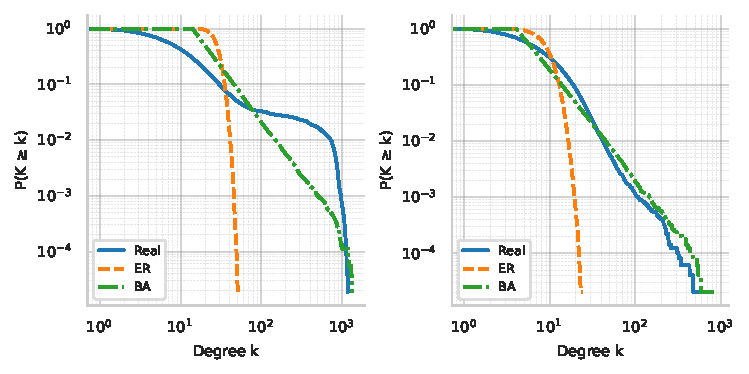
\includegraphics[width=0.9\linewidth]{img/B_degree_ccdf_vs_null.pdf}
\caption{Complementary CDF of degree on a log-log scale for $G_{BC}$ (left) and
$G_{Cit}$ (right), compared against ER and BA null models (dashed).
$G_{BC}$'s tail extends further, consistent with its lower fitted exponent $\hat{\gamma}=2.13$ vs $3.54$.}
\label{fig:degree_null}
\end{figure}

\newpage

\subsection{Centrality Analysis}\label{sec:centrality}
These graph-level properties arise from an uneven distribution of structural roles across nodes. BC's path-shortening effect raises closeness ($\bar{c}$: 0.0870 $\to$ 0.1017); added parallel routes simultaneously dilute betweenness ($\bar{b}$: $2.20 \to 1.69 \times 10^{-4}$, maximum: 0.0666 $\to$ 0.0502). The three measures respond differently at the distributional level (Table~\ref{tab:centrality}): degree and betweenness produce 1\,391 and 970 outliers beyond $\mu+2\sigma$, while closeness yields only 269. Closeness is bounded by global path structure and concentrates in a narrow range (${\approx}0.05$--$0.15$) in both graphs, with no heavy tail.

Rank correlation is moderate to strong ($\rho = 0.78$--$0.85$, Figure~\ref{fig:centrality_all}), yet the top of each ranking is almost entirely reshuffled. Degree overlap at top-10 is zero; closeness reaches just 1/10; even at top-100, both remain negligible (4 and 3 respectively). Betweenness is the exception: 3/10 at top-10 and 44/100 at top-100---key brokers retain their structural role across both graphs. Degree in $G_{BC}$ ranks papers by shared-reference exposure; degree in $G_{Cit}$ by incoming citations---so which graph is analysed determines which collaboration gaps become visible.

\begin{table}[hb]
\centering\footnotesize
\begin{tabular}{@{}lrrrrr@{}}
\toprule
 & Mean & Std & Max & P99 & $>\mu+2\sigma$ \\
\midrule
\multicolumn{6}{@{}l}{\textit{Combined LCC}} \\
\quad Degree      & 27.69   & 103.21  & 1\,169 & 726     & 1\,391 \\
\quad Betweenness & 1.69e-4 & 7.20e-4 & 0.0502 & 2.41e-3 &    970 \\
\quad Closeness   & 0.1017  & 0.0135  & 0.1435 & 0.1263  &    269 \\
\midrule
\multicolumn{6}{@{}l}{\textit{Citation LCC}} \\
\quad Degree      & 8.51    & 10.78   & 621    & 41      & 1\,194 \\
\quad Betweenness & 2.20e-4 & 1.02e-3 & 0.0666 & 3.38e-3 &    857 \\
\quad Closeness   & 0.0870  & 0.0131  & 0.1270 & 0.1107  &    180 \\
\bottomrule
\end{tabular}
\caption{Centrality statistics (NetworKit, undirected LCC) for $G_{BC}$ and $G_{Cit}$. $>\mu+2\sigma$: node count above two std devs.}
\label{tab:centrality}
\end{table}
\begin{figure}[h]
    \centering
    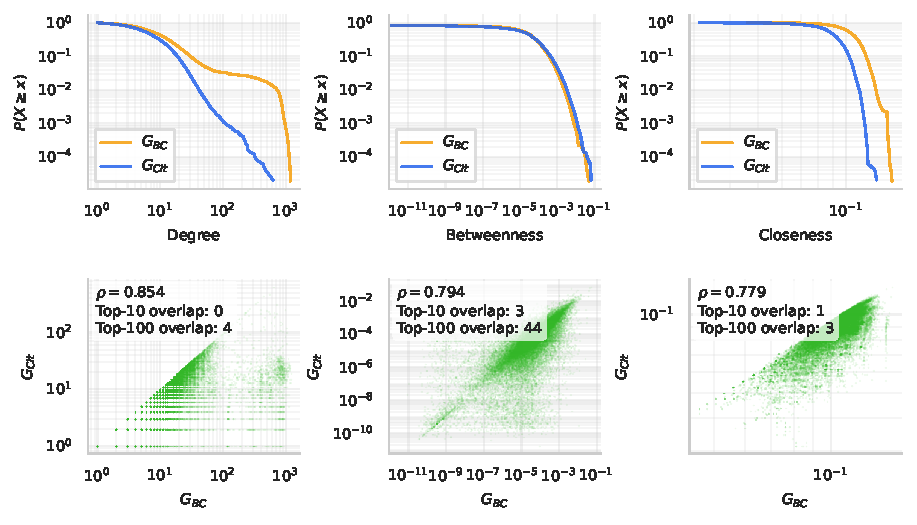
\includegraphics[width=\linewidth]{img/B_centrality_all.pdf}
    \caption{Log-log CCDF (top) and cross-graph scatter with Spearman $\rho$ and top-$k$ overlap (bottom), for degree (left), betweenness (center), and closeness (right).}
    \label{fig:centrality_all}
\end{figure}
